\section{Introduction}
\label{sec:introduction}


\par The objective of this laboratory assignment was to create a circuit that would transform an input AC voltage of amplitude 230V and frequency of 50 Hz to an output DC voltage of amplitude 12V and frequency 50Hz.To do this an Envelope detector, a Voltage Regulator and a Transformer were used. This last component was not actually modeled in the simulation and theorethical analysis. It was considerared that the transformer would be represented whith an alternated voltage source that would connect to the envelope detector and would reduce the amplitude of the first source in a ratio of n:1.This ratio will be decided during the simulation and theorethical analysis.\par
To determine whether or not the circuit was good when compared to others a merit classification sistem was created. This merit sistem took into account the cost of the components used and the ripple and average amplitude of the output voltage.The merit of the circuit will determined according to the following equation: 
\begin {equation}
	MERIT = \dfrac{1}{cost*(ripple_reg + abs(average_reg - 12) + 1e-6)}	
	\label{eq:i1}
\end{equation}

and the cost of the componets are the following: cost of resistors = 1 monetary unit (MU) per kOhm, cost of capacitors = 1 MU/uF
and cost of diodes = 0.1 MU per diode. The voltage source that represents the transformer was not taken into account in the cost. 
 
The circuit that was implemented can be seen in \textbf{Figure~\ref{fig:circuit_t3}}.\par
\begin{figure}[h] \centering
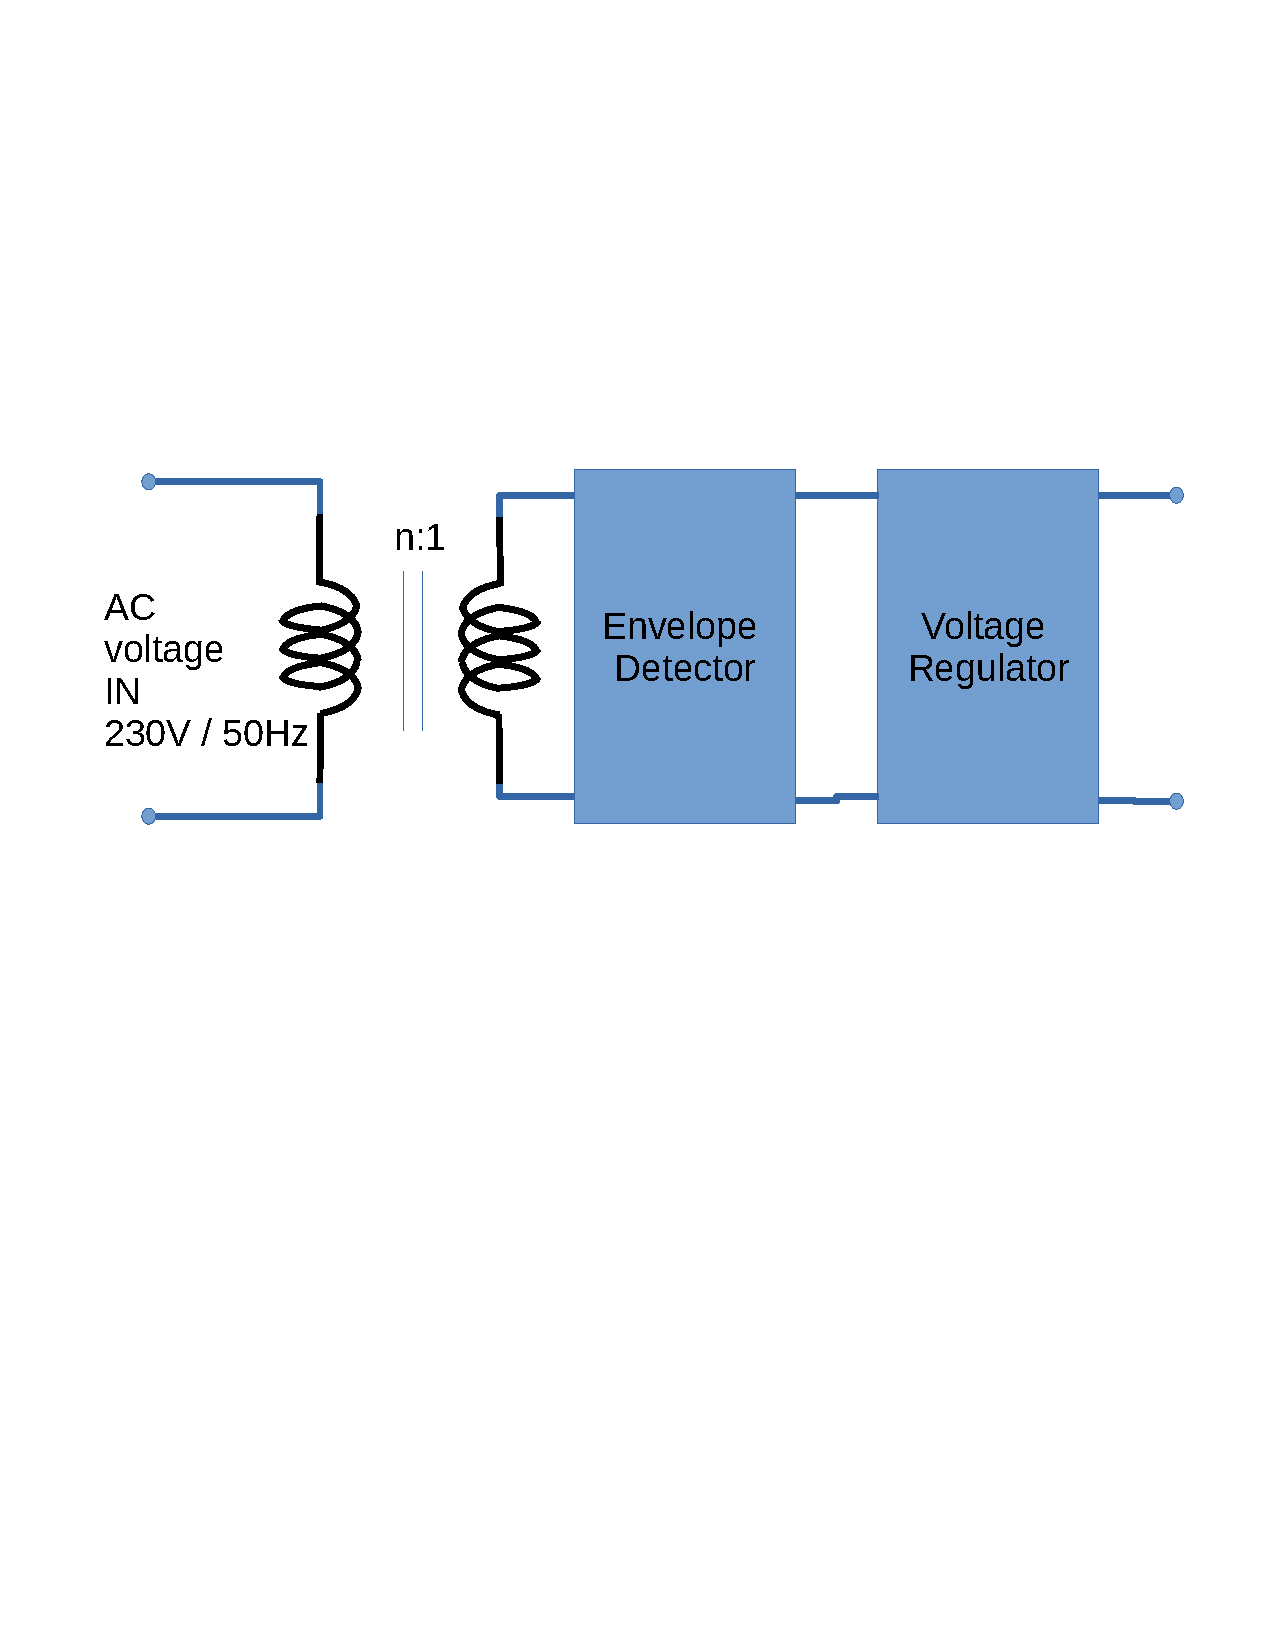
\includegraphics[width=0.6\linewidth]{circuit_t3.pdf}
\caption{Circuit in study}
\label{fig:circuit_t3}
\end{figure}


In this circuit there is also a linearly dependent voltage and current source. The circuit also contains 7 resistors.\par
The nodes of the circuit were numbered arbitrarily (from {\it$V_{0}$}  to {\it$V_{7}$} ), and it was considered that {\it node 0} was the ground node. The voltage-controlled current source {\it $I_b$} has a linear dependence on Voltage {\it $V_b$}, of constant {\it $K_b$}. The voltage {\it $V_b$} is the voltage drop at the ends of resistor {\it $R_3$}. The current-controlled voltage source {\it $V_d$} has a linear dependece on current {\it $I_d$}, of constant {\it $K_d$}. The control current {\it $I_d$} is the current that passes through the resistor {\it $R_6$}.
 

In Section~\ref{sec:analysis}, a theoretical analysis of the circuit is
presented. Here the circuit is analised for $t<0$ using the nodal analysis and the equivalent resistence $R_{eq}$ as seen from the capacitor terminals is determined. In this section both the natural and forced solutions for $V_6$ are also determined as well as the frequency responses for $V_c, V_s$ and $V_6 $. In Section~\ref{sec:simulation}, the circuit is analysed by
simulation using the program Ngspice. An operating point analysis is used to analyse the circuit when $t<0$ and another one to determine the time constant.A transient analysis is used to determine the natural and forced responses on node 6. A frequency analysis is also performed on node 6. The conclusions of this study are outlined in
Section~\ref{sec:conclusion}, where the theoretical results obtained in
Section~\ref{sec:analysis} are compared to the simulation results obtained in
Section~\ref{sec:simulation}.



%\begin{table}[h]
% \centering
 % \begin{tabular}{|l|r|}
  %  \hline    
   % {\bf Name} & {\bf Python-generated values} \\ \hline
	%R1 &  1.04606282456 \\ \hline
	%R2 &  2.00732621328 \\ \hline
	%R3 &  3.06060705885 \\ \hline
	%R4 &  4.07055531265 \\ \hline
	%R5 &  3.1225213804 \\ \hline
	%R6 &  2.06927045958 \\ \hline
	%R7 &  1.01531018068 \\ \hline
	%Va &  5.24359648479 \\ \hline
	%Id &  1.01891541651 \\ \hline
	%Kb &  7.0473187437 \\ \hline
	%Kc &  8.3479788681 \\ 
	%\hline

  %\end{tabular}
  %\caption{The variables that start with an {\it R} are the values of the resistors 
    %and are expressed in  kiloohm  (kOhm); the variable {\it Va} is a {\it voltage} and is expressed in
    %Volt (V) and the variable {\it Id}  is a {\it current} and expressed in
   %miliAmpere (mA). The constants {\it Kc} and {\it Kb} are  expressed in
   %kiloOhm  (kOhm) and miliSiemens (mS), respectively.}
  %\label{tab:python_values}
%\end{table}


\pagebreak

